%----------------------------------------------------------------------------------------
%	PACKAGES AND DOCUMENT CONFIGURATIONS
%----------------------------------------------------------------------------------------

\documentclass[10pt,a4paper]{article}
\usepackage[utf8]{inputenc}
\usepackage{graphicx} % Required for the inclusion of images
\graphicspath{{res/}}
\usepackage{natbib} % Required to change bibliography style to APA
\usepackage{amsmath} % Required for some math elements 
\usepackage{amsfonts}
\usepackage{amssymb}
\usepackage{listings}
\usepackage[T1,T2A]{fontenc}

\setlength\parindent{0pt} % Removes all indentation from paragraphs

\renewcommand{\labelenumi}{\alph{enumi}.} % Make numbering in the enumerate environment by letter rather than number (e.g. section 6)

%----------------------------------------------------------------------------------------
%	DOCUMENT INFORMATION
%----------------------------------------------------------------------------------------

\title{Утилита для исследования сети и сканер портов Nmap} % Title

\author{Виктор \textsc{Борисов}} % Author name

\date{\today} % Date for the report

\begin{document}

\maketitle % Insert the title, author and date

\newpage

\tableofcontents

\newpage

%----------------------------------------------------------------------------------------
%	SECTION 1
%----------------------------------------------------------------------------------------

\section{Цель работы}

Научиться работать с Nmap


%----------------------------------------------------------------------------------------
%	SECTION 2
%----------------------------------------------------------------------------------------

\section{Описание}

\textbf{nmap} — свободная утилита, предназначенная для разнообразного настраиваемого сканирования IP-сетей с любым количеством объектов, определения состояния объектов сканируемой сети (портов и соответствующих им служб). Изначально программа была реализована для систем UNIX, но сейчас доступны версии для множества операционных систем.

Nmap использует множество различных методов сканирования, таких как UDP, TCP (connect), TCP SYN (полуоткрытое), FTP-proxy (прорыв через ftp), Reverse-ident, ICMP (ping), FIN, ACK, Xmas tree, SYN- и NULL-сканирование. Nmap также поддерживает большой набор дополнительных возможностей, а именно: определение операционной системы удалённого хоста с использованием отпечатков стека TCP/IP, «невидимое» сканирование, динамическое вычисление времени задержки и повтор передачи пакетов, параллельное сканирование, определение неактивных хостов методом параллельного ping-опроса, сканирование с использованием ложных хостов, определение наличия пакетных фильтров, прямое (без использования portmapper) RPC-сканирование, сканирование с использованием IP-фрагментации, а также произвольное указание IP-адресов и номеров портов сканируемых сетей.
 
%----------------------------------------------------------------------------------------
%	SECTION 3
%----------------------------------------------------------------------------------------

\section{Ход работы}

\subsection{Поиск активных хостов}
\label{find_active_hosts}

Сканируем локальную сеть и ищем активные хосты с помощью команды nmap с ключом -sn и диапазоном ip адресов
\begin{verbatim}
$ nmap -sn 192.168.100.0/24
\end{verbatim}

Результат выполнения представлен на Рисунке \ref{fig:find_hosts}

\begin{figure}[h]
\begin{center}
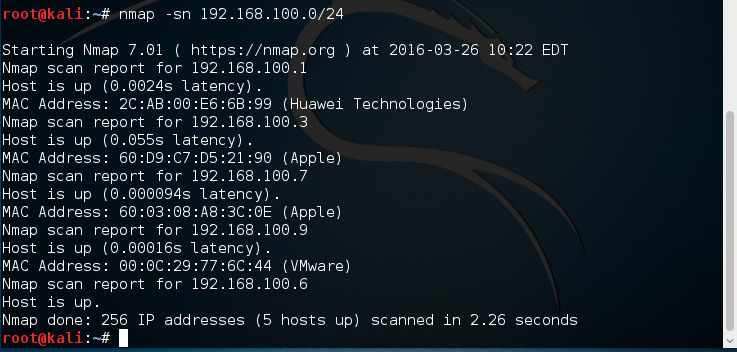
\includegraphics[width=0.65\textwidth]{find_hosts}
\caption{Поиск активных хостов.}
\label{fig:find_hosts}
\end{center}
\end{figure}

\subsection{Определение открытых портов}
\label{open_ports}

Для определения открытых портов необходимо воспользоваться командой
\begin{verbatim}
$ nmap --open адресХоста
\end{verbatim}

Результат выполнения для устройства под управлением ОС Linux представлен на Рисунке \ref{fig:open_ports_linux}, для iOS - Рисунок  \ref{fig:open_ports_iOS}

\begin{figure}[h]
\begin{center}
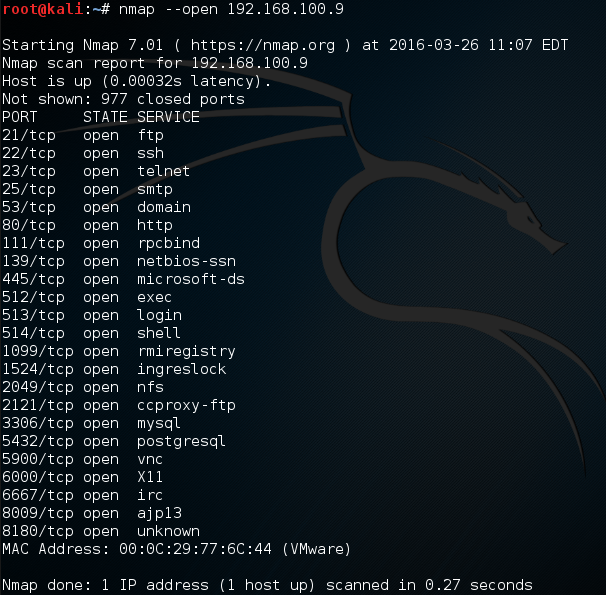
\includegraphics[width=0.65\textwidth]{open_ports_linux}
\caption{Открытые порты ОС Linux.}
\label{fig:open_ports_winOS}
\end{center}
\end{figure}

\begin{figure}[h]
\begin{center}
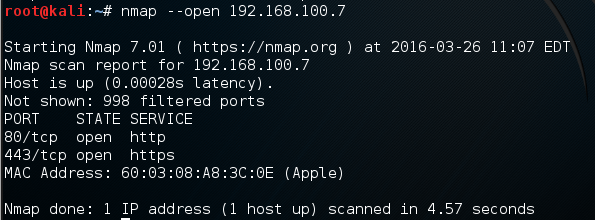
\includegraphics[width=0.65\textwidth]{open_ports_iOS}
\caption{Открытые порты ОС iOS.}
\label{fig:open_ports_iOS}
\end{center}
\end{figure}


\subsection{Определение версии сервисов}
\label{open_ports}

Для определения версии необходимо воспользоваться командой
\begin{verbatim}
$ nmap -sV адресХоста
\end{verbatim}

Результат выполнения для устройства под управлением ОС Windows представлен на Рисунке \ref{fig:service_version}

\begin{figure}[h]
\begin{center}
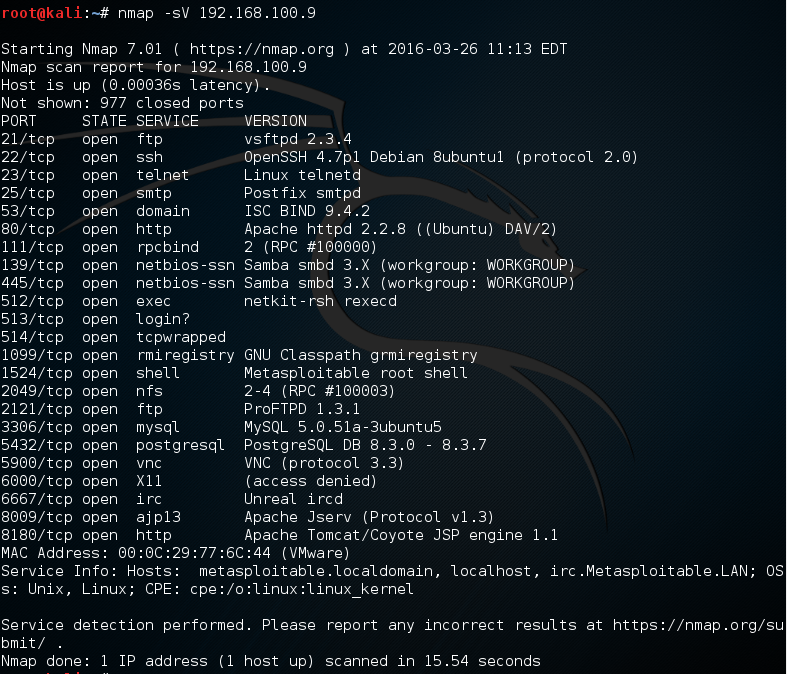
\includegraphics[width=0.65\textwidth]{service_version}
\caption{Версии сервисов.}
\label{fig:service_version}
\end{center}
\end{figure}

\subsection{nmap-services, nmap-os-db, nmap-service-probes}
\label{files}

Файл \textbf{nmap-services} содержит сопоставление имен портов с их номером и протоколом. Каждая запись содержит вероятность того, что порт открыт. Пример записей:
\begin{verbatim}
msp          18/udp    0.000610  # Message Send Protocol
chargen      19/tcp    0.002559  # ttytst source Character Generator
chargen      19/udp    0.015865  # ttytst source Character Generator
ftp-data     20/tcp    0.001079  # File Transfer [Default Data]
ftp-data     20/udp    0.001878  # File Transfer [Default Data]
ftp          21/tcp    0.197667  # File Transfer [Control]
ftp          21/udp    0.004844  # File Transfer [Control]
ssh          22/tcp    0.182286  # Secure Shell Login
ssh          22/udp    0.003905  # Secure Shell Login
telnet       23/tcp    0.221265
telnet       23/udp    0.006211
priv-mail    24/tcp    0.001154  # any private mail system
priv-mail    24/udp    0.000329  # any private mail system
smtp         25/tcp    0.131314  # Simple Mail Transfer
smtp         25/udp    0.001285  # Simple Mail Transfer
\end{verbatim}


Файл \textbf{nmap-os-db} необходим для определения ОС хоста. В ней содержится примеры ответов различных ОС на специальные запросы Nmap. Он разделен на блоки, так называемые отпечатки, содержащие название ОС, классификацию и данные ответа. Пример:

\begin{verbatim}
Fingerprint Linux 2.6.17 - 2.6.24
Class Linux | Linux | 2.6.X | general purpose
SEQ(SP=A5-D5%GCD=1-6%ISR=A7-D7%TI=Z%II=I%TS=U)
OPS(O1=M400C%O2=M400C%O3=M400C%O4=M400C%O5=M400C%O6=M400C)
WIN(W1=8018%W2=8018%W3=8018%W4=8018%W5=8018%W6=8018)
ECN(R=Y%DF=Y%T=3B-45%TG=40%W=8018%O=M400C%CC=N%Q=)
T1(R=Y%DF=Y%T=3B-45%TG=40%S=O%A=S+%F=AS%RD=0%Q=)
T2(R=N)
T3(R=Y%DF=Y%T=3B-45%TG=40%W=8018%S=O%A=S+%F=AS%O=M400C%RD=0%Q=)
T4(R=Y%DF=Y%T=3B-45%TG=40%W=0%S=A%A=Z%F=R%O=%RD=0%Q=)
T5(R=Y%DF=Y%T=3B-45%TG=40%W=0%S=Z%A=S+%F=AR%O=%RD=0%Q=)
T6(R=Y%DF=Y%T=3B-45%TG=40%W=0%S=A%A=Z%F=R%O=%RD=0%Q=)
T7(R=Y%DF=Y%T=3B-45%TG=40%W=0%S=Z%A=S+%F=AR%O=%RD=0%Q=)
U1(DF=N%T=3B-45%TG=40%IPL=164%UN=0%RIPL=G%RID=G%RIPCK=G%RUCK=G%RUD=G)
IE(DFI=N%T=3B-45%TG=40%CD=S)
\end{verbatim}

Файл \textbf{nmap-service-probes} содержит "пробы", используемые для определения программ по прослушиваемому порту (ключи -sV и -A). Пример:

\begin{verbatim}
##############################NEXT PROBE##############################
# DNS Server status request: http://www.rfc-editor.org/rfc/rfc1035.txt
Probe UDP DNSStatusRequest q|\0\0\x10\0\0\0\0\0\0\0\0\0|
ports 53,135
match domain m|^\0\0\x90\x04\0\0\0\0\0\0\0\0|
# This one below came from 2 tested Windows XP boxes
match msrpc m|^\x04\x06\0\0\x10\0\0\0\0\0\0\0|
[...]
##############################NEXT PROBE##############################
Probe UDP Help q|help\r\n\r\n|
ports 7,13,37
match chargen m|@ABCDEFGHIJKLMNOPQRSTUVWXYZ|
match echo m|^help\r\n\r\n$|
match time m|^[\xc0-\xc5]...$|
\end{verbatim}

\subsection{Добавление сигнатур в nmap-service-probes}
\label{add_probe}

Можно добавить собственную пробу в файл \textbf{nmap-service-probes}. Для этого необходимо знание хотя бы следующих конструкций:

\begin{enumerate}

\item

Директива Probe

Синтаксис: 
Probe <protocol> <probename> <probestring> \\
<protocol> - название протокола (TCP or UDP) \\
<probename> - имя пробы \\
<probestring> - отправляемое сообщение \\

\item
Директива match (для сопоставления ответа)
 
Синтаксис:

match <service> <pattern> [<versioninfo>]

<service> - название сервиса

<pattern> - шаблон ответа

<versioninfo> - информация о версии

\item


\end{enumerate}

Добавим в файл следующую пробу

\begin{verbatim}
##############################NEXT PROBE##############################
# Detects Borisov Victor service
Probe TCP BVService q|is_it_test_tcp_server|
ports 6792
match borisovvictorservice m|^yes_it_is| p/Borisov Victor/ 
\end{verbatim}

Создим и на исследуемом компьютере запустим TCP сервер, который слушает порт 6792 и в случае получение получение сообщения "is\_it\_test\_tcp\_server" отправляет обратно "yes\_it\_is".

Запустим проверку версии сервисов
\begin{verbatim}
nmap -sV 192.168.100.7
\end{verbatim}

На Рисунке \ref{fig:new_probe} отображен результат выполнения команды, на Рисунке \ref{fig:tcp_server} - вывод TCP сервера

\begin{figure}[h]
\begin{center}
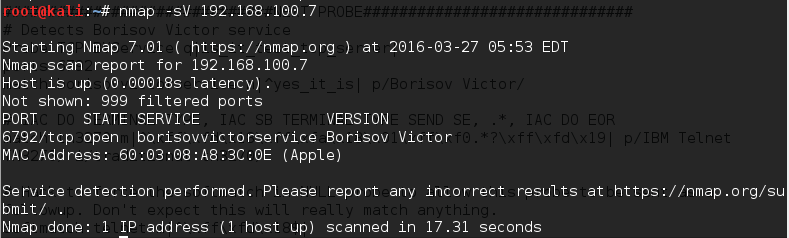
\includegraphics[width=0.65\textwidth]{new_probe}
\caption{Новый сервис.}
\label{fig:new_probe}
\end{center}
\end{figure}

\begin{figure}[h]
\begin{center}
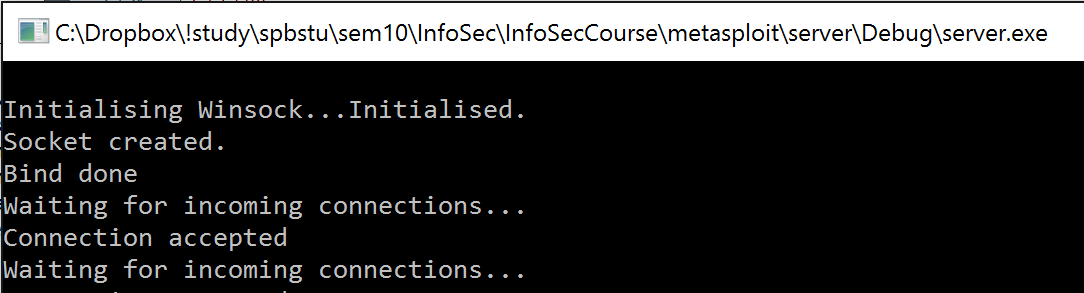
\includegraphics[width=0.65\textwidth]{tcp_server}
\caption{TCP сервер.}
\label{fig:tcp_server}
\end{center}
\end{figure}

\subsection{Сохранение вывода в xml}
\label{xml_output}

Для сохранения вывода утилиты в файл xml необходимо воспользоваться \textbf{-oX <file>}. Например,
\begin{verbatim}
nmap -sV 192.168.100.7 -oX /home/nmap_sv_1.xml
\end{verbatim}

\subsection{Исследование работы Nmap с помощью Wireshark}
\label{wireshark}

Для исследования сетевой активности nmap воспользуемся утилитой Wireshark. Для примера отследим пакеты относящиеся к определения TCP сервиса, написанного нами ранее.

На Рисунках \ref{fig:wireshark_1}, \ref{fig:wireshark_2} отображены TCP пакеты для определения версии сервиса. В исходящем пакете в передаваемых данных можно наблюдать текст "it\_it\_test\_tcp\_server", а в ответном пакете - "yes\_it\_is".

\begin{figure}[h]
\begin{center}
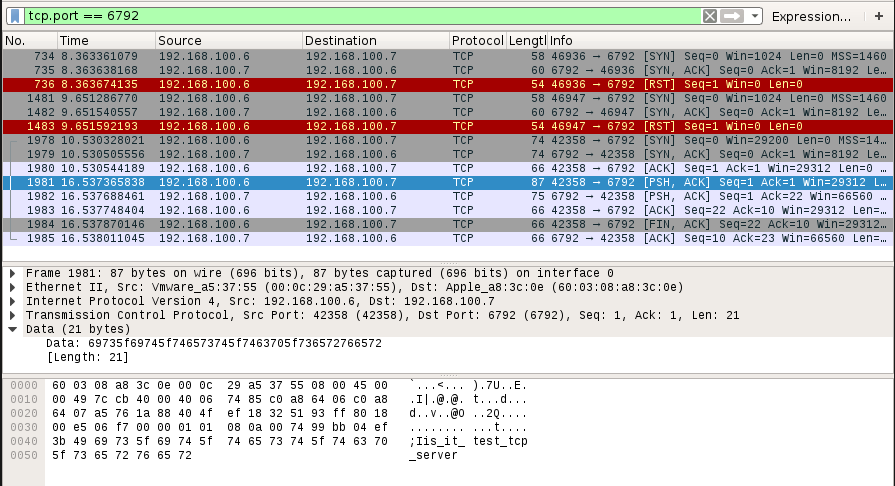
\includegraphics[width=0.65\textwidth]{wireshark_1}
\caption{Исходящий TCP пакет.}
\label{fig:wireshark_1}
\end{center}
\end{figure}

\begin{figure}[h]
\begin{center}
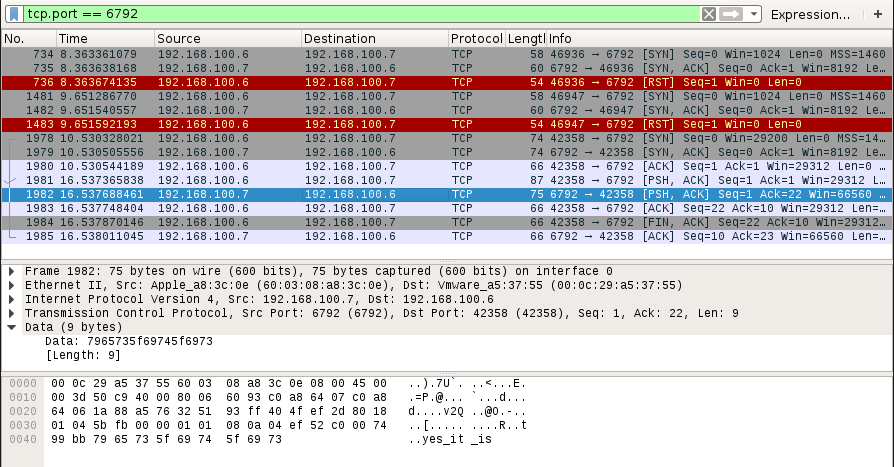
\includegraphics[width=0.65\textwidth]{wireshark_2}
\caption{Входящий TCP пакет.}
\label{fig:wireshark_2}
\end{center}
\end{figure}

\subsection{Metasploit Framework}
\label{msf}

- инструмент для создания, тестирования и использования эксплойтов. Позволяет конструировать эксплойты с необходимой в конкретном случае «боевой нагрузкой» (payloads), которая выполняется в случае удачной атаки, например, установка shell или VNC сервера. Также фреймворк позволяет шифровать шеллкод, что может скрыть факт атаки от IDS или IPS. Для проведения атаки необходима информация об установленных на удаленном сервере сервисах и их версии, то есть нужно дополнительное исследование с помощью таких инструментов, как nmap или nessus.

Проверим на уязвимости виртуальную машину Metasploitable2, используя db\_nmap (аналог nmap, сохраняющий результаты в БД) командой

\begin{verbatim}
db_nmap -A 192.168.100.9
\end{verbatim}

Результат сканирования отображен на Рисунках \ref{fig:db_nmap_1}, \ref{fig:db_nmap_2}, \ref{fig:db_nmap_3}

\begin{figure}[h]
\begin{center}
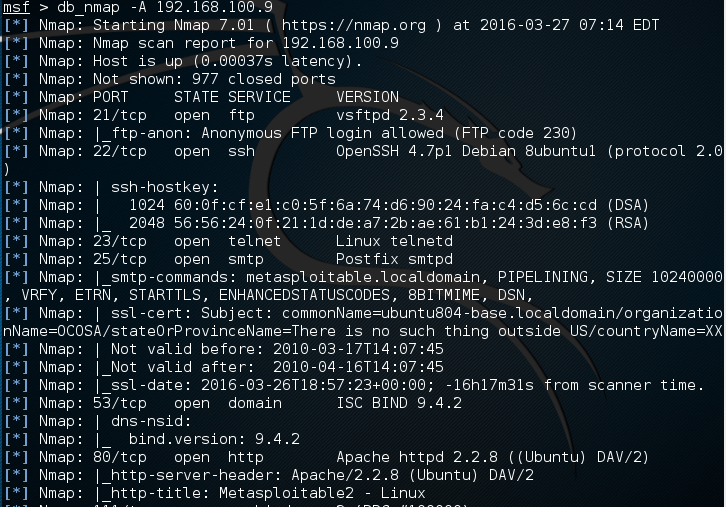
\includegraphics[width=0.8\textwidth]{db_nmap_1}
\caption{db\_nmap}
\label{fig:db_nmap_1}
\end{center}
\end{figure}

\begin{figure}[h]
\begin{center}
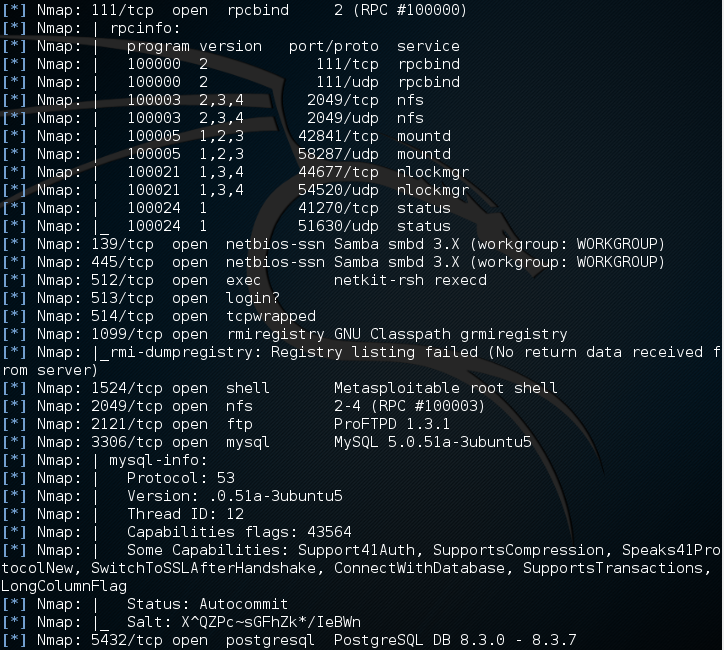
\includegraphics[width=0.8\textwidth]{db_nmap_2}
\caption{db\_nmap}
\label{fig:db_nmap_2}
\end{center}
\end{figure}

\begin{figure}[h]
\begin{center}
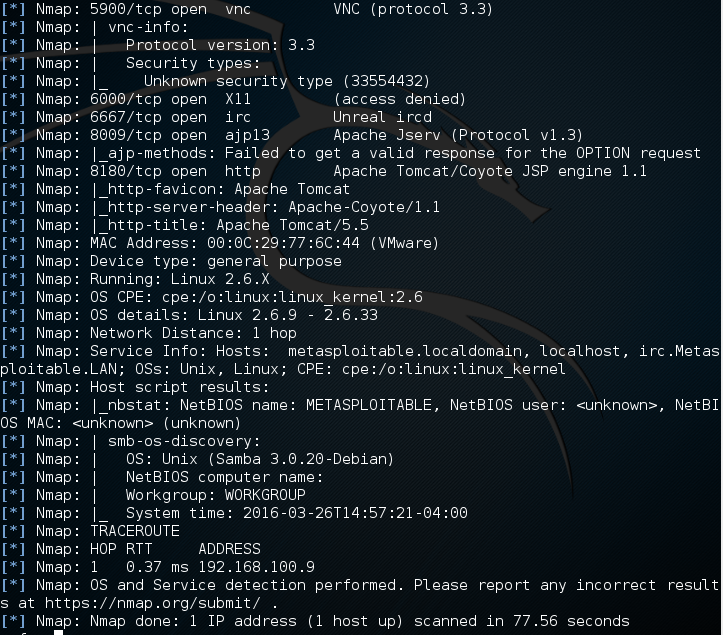
\includegraphics[width=0.8\textwidth]{db_nmap_3}
\caption{db\_nmap}
\label{fig:db_nmap_3}
\end{center}
\end{figure}

\subsection{Примеры записей из nmap-service-probes}
\label{probes_example}

\begin{verbatim}
##############################NEXT PROBE##############################
# Detects TN3270 Servers which send IAC DO TTYPE on initial connection
# instead of IAC DO TN3270E
Probe TCP tn3270 q|\xff\xfb\x18\xff\xfa\x18\x00IBM-3279-4-E\xff\xf0|
rarity 8
ports 23,2323,2023,623
sslports 992
\end{verbatim}

Согласно данной записи nmap для обнаружения сервиса использует протокол tcp для отправки пакета, содержащего \begin{verbatim}\xff\xfb\x18\xff\xfa\x18\x00IBM-3279-4-E\xff\xf0\end{verbatim}
Целевые порты 23, 2323, 2023, 623, ssl - 992. rarity - индикатор того, насколько часто возвращаемые пакеты содержат полезную информацию.

\begin{verbatim}
##############################NEXT PROBE##############################
Probe UDP AndroMouse q|AMSNIFF|
rarity 9
ports 8888

match AndroMouse m|^GOTBACK$|s p/AndroMouse Android remote mouse server/
\end{verbatim}

Протокол - UDP, редкость полезных ответов - 9, порт - 8888.
Данные для отправки \begin{verbatim}AMSNIFF\end{verbatim}
Шаблон ответа \begin{verbatim}m|^GOTBACK$|s\end{verbatim}
Дополнительная информация - "AndroMouse Android remote mouse server"

\begin{verbatim}
##############################NEXT PROBE##############################
Probe UDP AirHID q|from:airhid|
rarity 9
ports 13246
match AirHID m|^andReceiver-\d+\.\d+\.\d+$|s p/AirHID Andrioid remote mouse server/
\end{verbatim}

Протокол - UDP, редкость полезных ответов - 9, порт - 13246.
Данные для отправки \begin{verbatim}from:airhid\end{verbatim}
Шаблон ответа \begin{verbatim}m|^andReceiver-\d+\.\d+\.\d+$|s\end{verbatim}
Дополнительная информация - "AirHID Andrioid remote mouse server"

\begin{verbatim}
##############################NEXT PROBE##############################
# Queries z/OS Network Job Entry
# Sends an NJE Probe with the following information (text is converted to EBCDIC):
# TYPE        = OPEN
# OHOST       = FAKE
# RHOST       = FAKE
# RIP and OIP = 0.0.0.0
# R           = 0
# Based on http://www-01.ibm.com/support/knowledgecenter/SSLTBW_2.1.0/com.ibm.zos.v2r1.hasa600/init.htm
Probe TCP NJE q|\xd6\xd7\xc5\xd5@@@@\xc6\xc1\xd2\xc5@@@@\0\0\0\0\xc6\xc1\xd2\xc5@@@@\0\0\0\0\0|
rarity 9
ports 175
sslports 2252
# If the port supports NJE it will respond with either a 'NAK' or 'ACK' in EBCDIC
match nje m|^\xd5\xc1\xd2| p/IBM Network Job Entry (JES)/
match nje m|^\xc1\xc3\xd2| p/IBM Network Job Entry (JES)/
\end{verbatim}

Протокол - TCP, редкость полезных ответов - 9, порт - 175, ssl порт - 2252.
Данные для отправки \begin{verbatim}\xd6\xd7\xc5\xd5@@@@\xc6\xc1\xd2\xc5@@@@\0\0\0\0\xc6\xc1\xd2\xc5@@@@\0\0\0\0\0\end{verbatim}
Шаблоны ответа 
\begin{verbatim}
\xd5\xc1\xd2
\xc1\xc3\xd2
\end{verbatim}
Дополнительная информация для обоих шаблонов - "IBM Network Job Entry (JES)"

\begin{verbatim}
##############################NEXT PROBE##############################
# Sends a ServerInfo PBC request to the Basho Riak distributed database
Probe TCP riak-pbc q|\0\0\0\x01\x07|
rarity 8
ports 8087
match riak-pbc m|^....\x08..(riak@[\w._-]+)..([\w._-]+)$|s p/Basho Riak/ v/$2/ h/$1/
\end{verbatim}

Протокол - TCP, редкость полезных ответов - 8, порт - 8087.
Данные для отправки \begin{verbatim}\0\0\0\x01\x07\end{verbatim}
Шаблоны ответа 
\begin{verbatim}
^....\x08..(riak@[\w._-]+)..([\w._-]+)$
\end{verbatim}
Дополнительная информация - "Basho Riak", версия и имя хоста получаются из регулярного выражения.

\subsection{Описание скрипта finger}
\label{finger_script}

В начале содержится описание скрипта

\begin{verbatim}
description = [[
Attempts to get a list of usernames via the finger service.
]]

author = "Eddie Bell"

license = "Same as Nmap--See https://nmap.org/book/man-legal.html"
\end{verbatim}

Категории, к которым принадлежит скрипт

\begin{verbatim}
categories = {"default", "discovery", "safe"}
\end{verbatim}

Пример вывода

\begin{verbatim}
---
-- @output
-- PORT   STATE SERVICE
-- 79/tcp open  finger
-- | finger:
-- | Welcome to Linux version 2.6.31.12-0.2-default at linux-pb94.site !
-- |  01:14am  up  18:54,  4 users,  load average: 0.14, 0.08, 0.01
-- |
-- | Login      Name                  Tty      Idle  Login Time   Where
-- | Gutek      Ange Gutek           *:0          -     Wed 06:19 console
-- | Gutek      Ange Gutek            pts/1   18:54     Wed 06:20
-- | Gutek      Ange Gutek           *pts/0       -     Thu 00:41
-- |_Gutek      Ange Gutek           *pts/4       3     Thu 01:06
\end{verbatim}

Подлючение библиотек

\begin{verbatim}
require "comm"
require "shortport"
\end{verbatim}

Проверка называется ли сервис "finger" или порт равен 79. 
\begin{verbatim}
portrule = shortport.port_or_service(79, "finger")
\end{verbatim}

nmap.new\_try создает обработчик исключений, comm.exchange - обрабатывает сетевые транзакции. В данном случае просиходит ожидание пока не получено хотя бы 100 строк, не менее 5 секунд или пока хост не закроет подлючение.

\begin{verbatim}
action = function(host, port)
	local try = nmap.new_try()

	return try(comm.exchange(host, port, "\r\n",
        	{lines=100, proto=port.protocol, timeout=5000}))
end
\end{verbatim}


%----------------------------------------------------------------------------------------
%	END
%----------------------------------------------------------------------------------------


\end{document}

